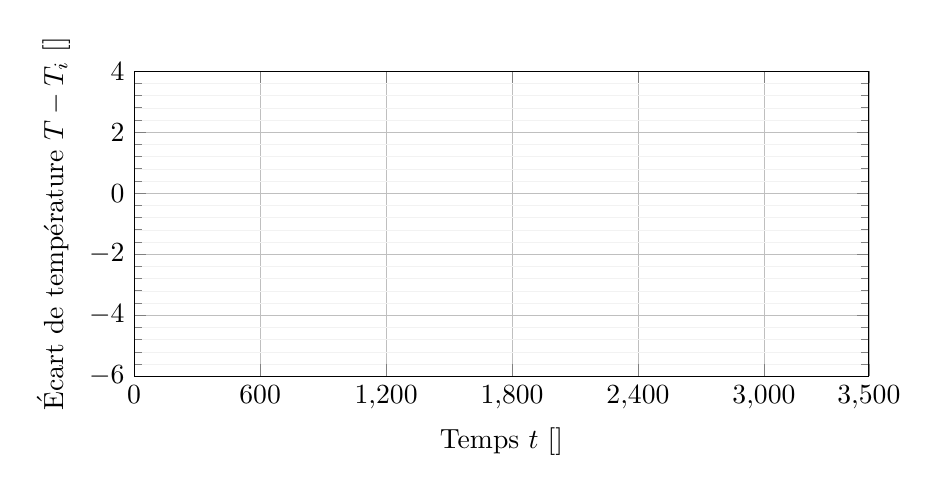
\begin{tikzpicture}
    \def\width{.9*\textwidth};
    \def\height{.5*\width};
    \def\legx{.5cm};
    \def\legy{\legx};
    
    \begin{axis}[width={\width},height={\height},grid=both,minor tick num=4,
    grid style={line width=.1pt, draw=gray!10},
    major grid style={line width=.2pt,draw=gray!50},
    xlabel={Temps $t$ [\unit{\s}]},
    ylabel={\'Ecart de température $T-T_i$ [\unit{\degreeCelsius}]},
    xmin=0,xmax=3500,
	ymin=-6,ymax=4,
    xtick={0,600,1200,1800,2400,3000,3500},%ytick={0,9.1120/100000,1.4452/10000,2.5/10000,5/10000,1/1000},
    domain=0:100,
    legend style = {at={(.95,.05)},anchor = south east},legend columns=2
    ]
    	
		
        
%        \legend{\\ \\};
    \end{axis}
\end{tikzpicture}